\chapter{Introduction}

% This document describes fligh dynamics model used by the MScSim flight simulation software.

\section{Conventions}

Flight Dynamics Model uses International System of Units (SI) for all internal computations. It is clearly specified if other units are used.

All rotations and rotation related operations are considered to be a passive (alias) rotations.

\section{Coordinates Systems}

\subsection{Body Axis System}

Body Axis System is body-centered, body-fixed coordinate system, with the x\nobreakdash-axis positive forwards, the y\nobreakdash-axis positive right and the z\nobreakdash-axis positive downwards.

\begin{figure}
  \centering
  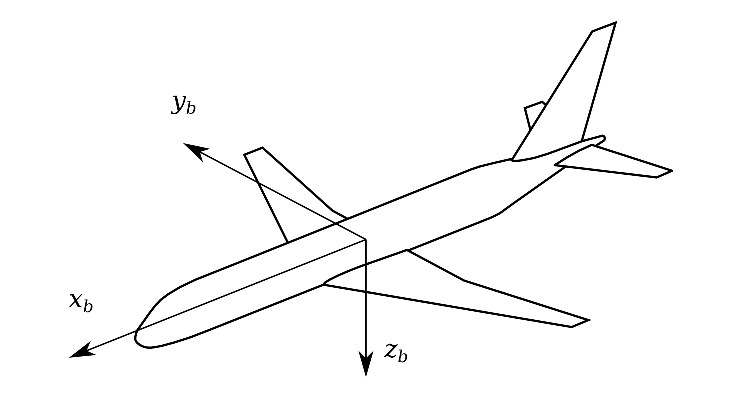
\includegraphics[width=110mm]{images/coordinate_system_BAS.eps}
  \caption{Body Axis System}
\end{figure}

\subsection{Stability Axis System}

Origin of the Stability Axis System is coincident with the origin of the Body Axis System, the x\nobreakdash-axis is directed along air freestream velocity vector projected onto the XZ plane of the Body Axis System, the y\nobreakdash-axis is coincident with the the y\nobreakdash-axis of the Body Axis System, and the z\nobreakdash-axis completes a right-handed coordinate system.

\begin{figure}
  \centering
  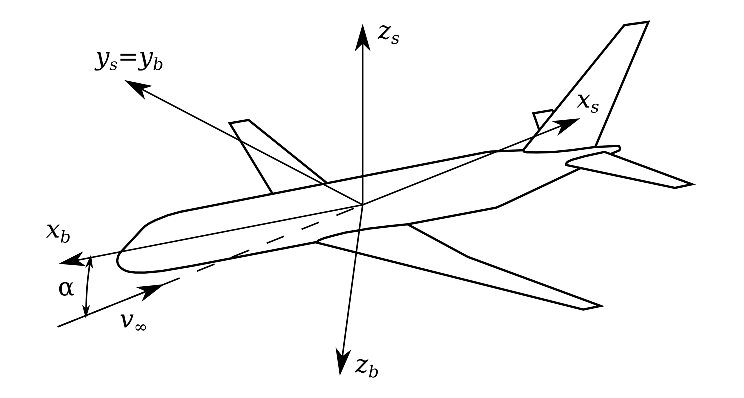
\includegraphics[width=110mm]{images/coordinate_system_Stab.eps}
  \caption{Stability Axis System}
\end{figure}

\subsection{Aerodynamic Axis System}

Origin of the Aerodynamic Axis System is coincident with the origin of the Body Axis System, the x\nobreakdash-axis is directed along air freestream velocity vector, the z\nobreakdash-axis lies in the aircraft plane of symmetry pointing upwards, and the y\nobreakdash-axis completes a right-handed coordinate system.

\begin{figure}
  \centering
  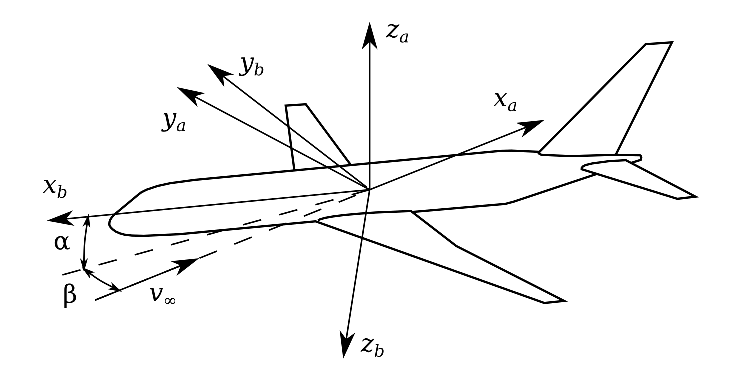
\includegraphics[width=110mm]{images/coordinate_system_Aero.eps}
  \caption{Aerodynamic Axis System}
\end{figure}

\subsection{Gravity Axis System}

There are basically two conventions of Gravity Axis Systems used for the purpose of flight dynamics East\nobreakdash-North\nobreakdash-Up and North\nobreakdash-East\nobreakdash-Down.

It is convenient to use North-East-Down axes system together with the Body Axis System and Bryant angles (Euler angles in z\nobreakdash-y\nobreakdash-x convention) as those angles in NED frame become aircraft heading, pitch and roll.

Considering all this, Gravity Earth Axis System is a coordinate system, with the x\nobreakdash-axis positive North, the y\nobreakdash-axis positive East and z\nobreakdash-axis positive downwards.

\subsection{Earth-fixed Axis System}

For any further considerations World Geodetic System 1984 as described in \cite{NIMA-TR-8350-2} is used as the Earth-fixed Axis System.

\begin{figure}
  \centering
  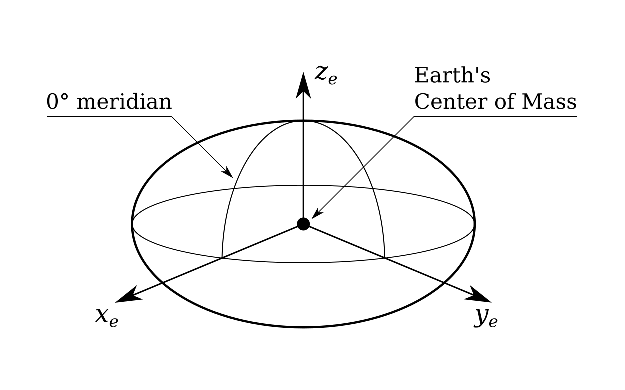
\includegraphics[width=90mm]{images/coordinate_system_WGS.eps}
  \caption{World Geodetic System 1984}
\end{figure}

\section{Aircraft Attitude}

\begin{figure}[h!]
  \centering
  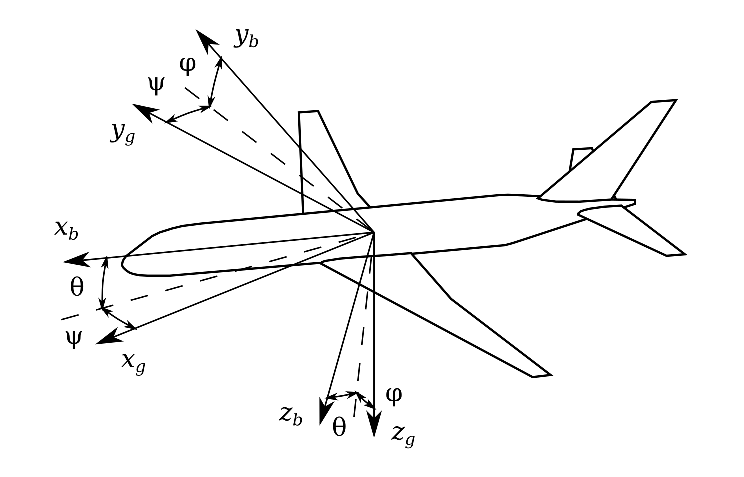
\includegraphics[width=110mm]{images/roll_pitch_yaw.eps}
  \caption{Tait–Bryan angles}
\end{figure}

Aircraft attitude is defined either by a quaternion or by quasi-Euler Tait-Bryan $\Psi$\nobreakdash-$\Theta$\nobreakdash-$\Phi$ angles in z\nobreakdash-y\nobreakdash-x convention. It is convenient to use such a convention, as this angles becomes aircraft roll, pitch and heading when expressed in North\nobreakdash-East\nobreakdash-Down coordinate system.

\section{Transformations Between Coordinates Systems}

\subsection{Rotation Matrices}

ransformation to the coordinate system rotated by Tait-Bryan $\Psi$\nobreakdash-$\Theta$\nobreakdash-$\Phi$ angles can be performed using rotation matrix, which is given by the following relations. \cite{Padfield2007, Sibilski2004}
\begin{align}
  \boldsymbol T \left( \Phi \right) &=
  \left[
    \begin{matrix}
      1 &          0 &         0 \\
      0 &  \cos \Phi & \sin \Phi \\
      0 & -\sin \Phi & \cos \Phi \\
    \end{matrix}
  \right]
  \\
  \boldsymbol T \left( \Theta \right) &=
  \left[
    \begin{matrix}
      \cos \Theta & 0 & -\sin \Theta \\
                0 & 1 &            0 \\
      \sin \Theta & 0 &  \cos \Theta \\
    \end{matrix}
  \right]
  \\
  \boldsymbol T \left( \Psi \right) &=
  \left[
    \begin{matrix}
       \cos\Psi & \sin\Psi & 0 \\
      -\sin\Psi & \cos\Psi & 0 \\
              0 &        0 & 1 \\
    \end{matrix}
  \right]
\end{align}

\begin{equation}
  \begin{array}{c}
  \boldsymbol T \left( \Phi,\Theta,\Psi \right) =
  \boldsymbol T \left( \Phi \right)
  \boldsymbol T \left( \Theta \right) 
  \boldsymbol T \left( \Psi \right) = \\
  \left[
    \begin{matrix}
       \cos \Theta \cos \Psi &
       \cos \Theta \sin \Psi &
      -\sin \Theta \\
       \cos \Psi   \sin \Phi   \sin \Theta - \cos \Phi   \sin \Psi &
       \cos \Phi   \cos \Psi + \sin \Phi     \sin \Theta \sin \Psi &
       \cos \Theta \sin \Phi \\
       \sin \Phi   \sin \Psi + \cos \Phi     \cos \Psi   \sin \Theta &
       \cos \Phi   \sin \Theta \sin \Psi   - \cos \Psi   \sin \Phi &
       \cos \Phi   \cos \Theta \\
    \end{matrix}
  \right]
  \end{array}
\end{equation}

\subsection{Geographic Coordinates}

\subsubsection{Conversion from Geographic to Cartesian Coordinates}

Procedure of conversion from geographic coordinates to the Cartesian coordinates system is given as follows.
\begin{align}
  e    &= \frac{1}{a} \sqrt{a^2-b^2} \\
  \chi &= \sqrt{ 1 - e^2 \sin^2 \varphi } \\
  x_e  &= \left( \frac{a}{\chi} + h \right) \cos \varphi \cos \lambda \\
  y_e  &= \left( \frac{a}{\chi} + h \right) \cos \varphi \sin \lambda \\
  z_e  &= \left( a \frac{1-e^2}{\chi} + h \right) \sin \varphi
\end{align}

\subsubsection{Conversion from Cartesian to Geographic Coordinates}

Reverse conversion is given as follows. \cite{Zhu1994}
\begin{align}
  r    &= \sqrt{x_e^2+y_e^2} \\
  E^2  &= a^2 - b^2 \\
  e'^2 &= \frac{a^2-b^2}{b^2} \\
  F    &= 54 b^2 z_e^2 \\
  G    &= r^2 + \left( 1 - e^2 \right) z_e^2 - e^2 E^2 \\
  C    &= \frac{e^4 F r^2}{G^3} \\
  S    &= \sqrt[3]{1+C+\sqrt{C^2+2C}} \\
  P_0  &= S + \frac{1}{S} + 1 \\
  P    &= \frac{F}{3P_0^2 G^2} \\
  Q    &= \sqrt{1 + 2e^4 P}
\end{align}

\begin{equation}
  r_0  =
  \frac{ -\left(Pe^2 r \right) }{1+Q}
  + \sqrt{
    \frac{1}{2}a^2 \left(1+\frac{1}{Q}\right)
    -
    \frac{P\left(1-e^2 \right)z_e^2}{Q+Q^2}
    -
    \frac{1}{2}Pr^2
  }
\end{equation}

% \begin{equation}
%   r_0  = \frac{-\left(Pe^2 r \right)}{1+Q} +\sqrt{\frac{1}{2}a^2 \left(1+\frac{1}{Q}\right) - \frac{P\left(1-e^2 \right)z_i^2}{Q+Q^2}-\frac{1}{2}Pr^2}
% \end{equation}

\begin{align}
  U_0  &= r - e^2 r_0 \\
  U    &= \sqrt{ U_0^2 + z_e^2 } \\
  V    &= \sqrt{ U_0^2 + \left( 1 - e^2 \right) z_e^2 } \\
  Z_0  &= \frac{b^2 z_e}{aV}
\end{align}

Geographic coordinates are given as.
\begin{align}
  h    &= U \left( 1 - \frac{b^2}{aV} \right) \\
  \varphi &= \arctan \left( \frac{z_e + e'^2 Z_0}{r} \right) \\
  \lambda &= \arctan \left( \frac{y_e}{z_e} \right)
\end{align}
